\gdef\Afill{white}

\gdef\ABOption{black}
\gdef\BCOption{black}
\gdef\CDOption{black}
\gdef\CEOption{black}
\gdef\CtOption{black}
\gdef\DtOption{black}
\gdef\ECOption{black}
\gdef\EFOption{black}
\gdef\EtOption{black}
\gdef\FGOption{black}
\gdef\GtOption{black}
\gdef\sAOption{black}
\gdef\sEOption{black}


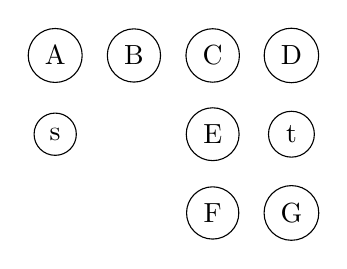
\begin{tikzpicture}{->, auto, node distance = 5cm}
\node[draw, circle, fill=\Afill] (A) at (0,0) {A};
\node[draw, circle, fill=\Afill] (B) [right of=A] {B};
\node[draw, circle, fill=\Afill] (C) [right of=B] {C};
\node[draw, circle, fill=\Afill] (D) [right of=C] {D};
\node[draw, circle, fill=\Afill] (E) [below of=C] {E};
\node[draw, circle, fill=\Afill] (F) [below of=E] {F};
\node[draw, circle, fill=\Afill] (G) [right of=F] {G};
\node[draw, circle, fill=\Afill] (s) [below of=A] {s};
\node[draw, circle, fill=\Afill] (t) [right of=E] {t};
\end{tikzpicture}